\documentclass[11pt,a4paper]{report}
\usepackage[utf8]{inputenc}
\usepackage{amsmath}
\usepackage{graphicx}
\usepackage{gensymb}
\usepackage{listings}
\usepackage{tikz}
\usepackage{pgfplots}
\usepackage{mathtools}
\usetikzlibrary{arrows,positioning}
\tikzset{
    %Define standard arrow tip
    >=stealth',
    % Define arrow style
    pil/.style={
           ->,
           thick,
           shorten <=2pt,
           shorten >=2pt,}
}
\usepackage{geometry}
\geometry{
    left=2cm,
    right=0.64cm,
    top=0.64cm,
    bottom=2cm
}
\usepackage{multicol}
\setlength{\columnsep}{1cm}
\graphicspath{ {images/} }

\begin{document}

\chapter{Semester 2 Examination 2012-2013\\CZ4034 Information Retrieval}
\begin{multicols*}{2}

\section{Question 1}

\noindent \textbf{Question 1a}

\begin{center}
\begin{tabular}{| l | l | l | l |}
    \hline
    Part      & Wilcard Query & Bigrams    & Permuterms \\
    \hline
    e.g       & SH*           & \$S, SH     & \$SH* \\
    (i)       & N*T*U         & \$N, T, U\$ & U\$N* \\
    (ii)      & S*T           & \$S, T\$    & T\$S* \\
    (iii)     & *H*T          & H, T\$      & T\$*  \\
    (iv)      & *H*           & H           & H*    \\
    (v)       & S*I*T         & \$S, I, T   & \$S*  \\
    \hline
\end{tabular}
\end{center}

\noindent For (i) (iii) and (v), after searching for terms using the permuterms, we do exhausted filter on each terms.\\

\noindent \textbf{Question 1b}

\noindent \textbf{(i)} Advantage 1: Permuterm is more efficient than bigram, for example, in Q1a(i) we need to do 2 search in two binary tree when using bigram approach, but we only need to do 1 search in 1 permuterm index when using permuterm approach.

\noindent Advantage 2: [Help wanted!]\\

\noindent \textbf{(ii)} The index size bigram is smaller than permuterm.\\

\noindent \textbf{(iii)} For bigram, we need to find intersection of terms in all result lists by using merging algorithm. For permuterms, we need to do exhausted filters for query with more than one *.\\

\noindent \textbf{Question 1c}

\noindent \textbf{(i)} Since the boolean expression is equivalent to \verb|NOT( X OR Y )|, the algorithm:

\begin{lstlisting}
define ALL_DATA
XY = Merge X and Y without duplication
Remove elements of XY from ALL_DATA
\end{lstlisting}

\noindent Note: the real answer should be longer than this, specifically, the last steps need to elaboration. \\

\noindent \textbf{(ii)} We need $O(x+y)$ complexity to merge X and Y. To remove $x+y$ data from a list with $n$ elements, we need $O((x+y)+n)$. Hence, the worse case complexity for the algorithm is $O(x+y+n)$.

\section{Question 2}

\noindent \textbf{Question 2a}

\noindent \textbf{(i)} Not in syllabus\\

\noindent \textbf{(ii)} Not in syllabus\\

\noindent \textbf{Question 2b}

\noindent \textbf{(i)} For SE1

$$\text{Precision@1}=1$$
$$\text{Precision@3}=2/3$$
$$\text{Precision@9}=3/9$$
$$\text{Precision@10}=4/10$$
$$\text{MAP} = \frac{1}{4} \cdot (1 + \frac{2}{3} + \frac{3}{9} + \frac{4}{10})= 0.60$$

\noindent For SE2:

$$\text{Precision@2}=1/2$$
$$\text{Precision@5}=2/5$$
$$\text{Precision@6}=3/6$$
$$\text{Precision@7}=4/7$$
$$\text{MAP} = \frac{1}{4} \cdot (\frac{1}{2} + \frac{2}{5} + \frac{3}{6} + \frac{4}{7}) = 0.49$$

\noindent \textbf{(ii)} For a given query topic $Q$, R-precision is the precision at $R$, where $R$ is the number of relevant documents for $Q$. In other words, if there are $r$ relevant documents among the top-R retrieved documents, then R-precision is $r/R$.\\

\noindent For this question, the R-precision for SE1 and SE2 are:

$$\text{SE1, Precision@4}=2/4$$
$$\text{SE2, Precision@4}=1/4$$

\noindent \textbf{(iii)} According to MAP of two search engine, SE1 is better because it has higher MAP. \\

\noindent \textbf{Question 2c}

\noindent \textbf{(i)} Not in syllabus\\

\noindent \textbf{(ii)} Not in syllabus\\

\noindent \textbf{(iii)} Not in syllabus

\section{Question 3}

\noindent \textbf{Question 3a}

\noindent \textbf{(i)} The number of vocabulary is 19, i.e. \verb|as|, \verb|back|, \verb|but|, \verb|can|, \verb|do|, \verb|expected|, \verb|food|, \verb|go|, \verb|good|, \verb|is|, \verb|long|, \verb|must|, \verb|nice|, \verb|not|, \verb|service|, \verb|to|, \verb|try|, \verb|wait|, \verb|want|.

$$ P(\text{as} | \text{Postive} ) = \frac{1+ 1}{17 + 19} = \frac{2}{36}$$
$$ P(\text{back} | \text{Postive} ) = \frac{1+ 1}{17 + 19} = \frac{2}{36}$$
$$ P(\text{but} | \text{Postive} ) = \frac{0+ 1}{17 + 19} = \frac{1}{36}$$
$$ P(\text{can} | \text{Postive} ) = \frac{1+ 1}{17 + 19} = \frac{2}{36}$$
$$ P(\text{do} | \text{Postive} ) = \frac{0+ 1}{17 + 19} = \frac{1}{36}$$
$$ P(\text{expected} | \text{Postive} ) = \frac{1+ 1}{17 + 19} = \frac{2}{36}$$
$$ P(\text{food} | \text{Postive} ) = \frac{2+ 1}{17 + 19} = \frac{3}{36}$$
$$ P(\text{go} | \text{Postive} ) = \frac{1+ 1}{17 + 19} = \frac{2}{36}$$
$$ P(\text{good} | \text{Postive} ) = \frac{1+ 1}{17 + 19} = \frac{2}{36}$$
$$ P(\text{is} | \text{Postive} ) = \frac{1+ 1}{17 + 19} = \frac{2}{36}$$
$$ P(\text{long} | \text{Postive} ) = \frac{0+ 1}{17 + 19} = \frac{1}{36}$$
$$ P(\text{must} | \text{Postive} ) = \frac{1+ 1}{17 + 19} = \frac{2}{36}$$
$$ P(\text{nice} | \text{Postive} ) = \frac{2+ 1}{17 + 19} = \frac{3}{36}$$
$$ P(\text{not} | \text{Postive} ) = \frac{1+ 1}{17 + 19} = \frac{2}{36}$$
$$ P(\text{service} | \text{Postive} ) = \frac{1+ 1}{17 + 19} = \frac{2}{36}$$
$$ P(\text{to} | \text{Postive} ) = \frac{1+ 1}{17 + 19} = \frac{2}{36}$$
$$ P(\text{try} | \text{Postive} ) = \frac{1+ 1}{17 + 19} = \frac{2}{36}$$
$$ P(\text{wait} | \text{Postive} ) = \frac{1+ 1}{17 + 19} = \frac{2}{36}$$
$$ P(\text{want} | \text{Postive} ) = \frac{0+ 1}{17 + 19} = \frac{1}{36}$$

$$ P(\text{as} | \text{Negative} ) = \frac{2 + 1}{21 + 19} = \frac{3}{40}$$
$$ P(\text{back} | \text{Negative} ) = \frac{1 + 1}{21 + 19} = \frac{2}{40}$$
$$ P(\text{but} | \text{Negative} ) = \frac{1 + 1}{21 + 19} = \frac{2}{40}$$
$$ P(\text{can} | \text{Negative} ) = \frac{0 + 1}{21 + 19} = \frac{1}{40}$$
$$ P(\text{do} | \text{Negative} ) = \frac{2 + 1}{21 + 19} = \frac{3}{40}$$
$$ P(\text{expected} | \text{Negative} ) = \frac{1 + 1}{21 + 19} = \frac{2}{40}$$
$$ P(\text{food} | \text{Negative} ) = \frac{1 + 1}{21 + 19} = \frac{2}{40}$$
$$ P(\text{go} | \text{Negative} ) = \frac{1 + 1}{21 + 19} = \frac{2}{40}$$
$$ P(\text{good} | \text{Negative} ) = \frac{1 + 1}{21 + 19} = \frac{2}{40}$$
$$ P(\text{is} | \text{Negative} ) = \frac{1 + 1}{21 + 19} = \frac{2}{40}$$
$$ P(\text{long} | \text{Negative} ) = \frac{1 + 1}{21 + 19} = \frac{2}{40}$$
$$ P(\text{must} | \text{Negative} ) = \frac{0 + 1}{21 + 19} = \frac{1}{40}$$
$$ P(\text{nice} | \text{Negative} ) = \frac{1 + 1}{21 + 19} = \frac{2}{40}$$
$$ P(\text{not} | \text{Negative} ) = \frac{3 + 1}{21 + 19} = \frac{4}{40}$$
$$ P(\text{service} | \text{Negative} ) = \frac{0 + 1}{21 + 19} = \frac{1}{40}$$
$$ P(\text{to} | \text{Negative} ) = \frac{2 + 1}{21 + 19} = \frac{3}{40}$$
$$ P(\text{try} | \text{Negative} ) = \frac{0 + 1}{21 + 19} = \frac{1}{40}$$
$$ P(\text{wait} | \text{Negative} ) = \frac{1 + 1}{21 + 19} = \frac{2}{40}$$
$$ P(\text{want} | \text{Negative} ) = \frac{2 + 1}{21 + 19} = \frac{3}{40}$$

\noindent \textbf{(ii)}
\begin{center}\verb|want to go back back|\end{center}

\scriptsize
$$P(\text{Positive}|d) = \frac{1}{P(d)} \frac{1}{36} \cdot \frac{2}{36} \cdot \frac{2}{36} \cdot (\frac{2}{36})^2 \cdot \frac{4}{7}= 0.151 \times 10^{-6}$$

$$P(\text{Negative}|d) = \frac{1}{P(d)} \frac{3}{40} \cdot \frac{3}{40} \cdot \frac{2}{40} \cdot (\frac{2}{40})^2  \cdot \frac{3}{7}= 0.301 \times 10^{-6}$$
\normalsize

\noindent Since $P(\text{Negative}|d) > P(\text{Positive}|d)$, we classify the review as Negative.\\

\noindent \textbf{(iii)} Before normalize
\scriptsize
\begin{center}
\begin{tabular}{| l | l l l l l l l |}
\hline
Term     & ID1 & ID2 & ID3 & ID4 & ID5 & ID6 & ID7 \\ \hline
as       & 0   & 1   & 0   & 0   & 2   & 0   & 0   \\
back     & 0   & 0   & 1   & 0   & 0   & 1   & 0   \\
but      & 0   & 0   & 0   & 0   & 1   & 0   & 0   \\
can      & 0   & 0   & 1   & 0   & 0   & 0   & 0   \\
do       & 0   & 0   & 0   & 0   & 0   & 1   & 1   \\
expected & 0   & 1   & 0   & 0   & 1   & 0   & 0   \\
food     & 1   & 1   & 0   & 0   & 1   & 0   & 0   \\
go       & 0   & 0   & 1   & 0   & 0   & 1   & 0   \\
good     & 0   & 1   & 0   & 0   & 1   & 0   & 0   \\
is       & 0   & 1   & 0   & 0   & 1   & 0   & 0   \\
long     & 0   & 0   & 0   & 0   & 0   & 0   & 1   \\
must     & 0   & 0   & 0   & 1   & 0   & 0   & 0   \\
nice     & 2   & 0   & 0   & 0   & 1   & 0   & 0   \\
not      & 0   & 0   & 1   & 0   & 1   & 1   & 1   \\
service  & 1   & 0   & 0   & 0   & 0   & 0   & 0   \\
to       & 0   & 0   & 1   & 0   & 0   & 1   & 1   \\
try      & 0   & 0   & 0   & 1   & 0   & 0   & 0   \\
wait     & 0   & 0   & 1   & 0   & 0   & 0   & 1   \\
want     & 0   & 0   & 0   & 0   & 0   & 1   & 1   \\ \hline
\end{tabular}
\end{center}
\normalsize

\noindent We do a normalization without TF-IDF (you can do TF-IDF too).

\scriptsize
\begin{center}
\begin{tabular}{| l | l l l l l l l |}
\hline
Term     & ID1  & ID2  & ID3  & ID4  & ID5  & ID6  & ID7 \\ \hline
as       & 0    & 0.45 & 0    & 0    & 0.60 & 0    & 0   \\
back     & 0    & 0    & 0.41 & 0    & 0    & 0.41 & 0   \\
but      & 0    & 0    & 0    & 0    & 0.30 & 0    & 0   \\
can      & 0    & 0    & 0.41 & 0    & 0    & 0    & 0   \\
do       & 0    & 0    & 0    & 0    & 0    & 0.41 & 0.41\\
expected & 0    & 0.45 & 0    & 0    & 0.30 & 0    & 0   \\
food     & 0.41 & 0.45 & 0    & 0    & 0.30 & 0    & 0   \\
go       & 0    & 0    & 0.41 & 0    & 0    & 0.41 & 0   \\
good     & 0    & 0.45 & 0    & 0    & 0.30 & 0    & 0   \\
is       & 0    & 0.45 & 0    & 0    & 0.30 & 0    & 0   \\
long     & 0    & 0    & 0    & 0    & 0    & 0    & 0.41\\
must     & 0    & 0    & 0    & 0.71 & 0    & 0    & 0   \\
nice     & 0.82 & 0    & 0    & 0    & 0.30 & 0    & 0   \\
not      & 0    & 0    & 0.41 & 0    & 0.30 & 0.41 & 0.41\\
service  & 0.41 & 0    & 0    & 0    & 0    & 0    & 0   \\
to       & 0    & 0    & 0.41 & 0    & 0    & 0.41 & 0.41\\
try      & 0    & 0    & 0    & 0.71 & 0    & 0    & 0   \\
wait     & 0    & 0    & 0.41 & 0    & 0    & 0    & 0.41\\
want     & 0    & 0    & 0    & 0    & 0    & 0.41 & 0.41\\ \hline
\end{tabular}
\end{center}
\normalsize

\noindent I do not finish the solution for this answer, it takes too long to finish. \\

\noindent \textbf{Question 3b}

\noindent For class A:
\begin{center}
\begin{tabular}{| l | l | l |}
\hline
             & Truth: Yes & Truth No \\ \hline
System: Yes  & 4  & 8 \\ \hline
System: No   & 10 & 28\\ \hline
\end{tabular}
\end{center}

\noindent For class B:
\begin{center}
\begin{tabular}{| l | l | l |}
\hline
             & Truth: Yes & Truth No \\ \hline
System: Yes  & 12 & 4  \\ \hline
System: No   & 8  & 26 \\ \hline
\end{tabular}
\end{center}

$$P_A = \frac{4}{12}$$
$$R_A = \frac{4}{14}$$
$$F_A = \frac{2PR}{P+R} = \frac{4}{13}$$

$$P_B = \frac{12}{16}$$
$$R_B = \frac{12}{20}$$
$$F_B = \frac{2PR}{P+R} = \frac{2}{3}$$

\noindent For macro-averaging, the weight is the same:

$$F = \frac{1}{2} \cdot \frac{4}{13} + \frac{1}{2} \cdot \frac{2}{3} = 0.487$$

\noindent For micro-averaging:

$$P = \frac{4 + 12}{12 + 16} = \frac{16}{28}$$
$$R = \frac{4 + 12}{14 + 20} = \frac{16}{34}$$
$$F = 0.516$$

\noindent \textbf{Question 3c}

\noindent Fist, we can solve the problem by collecting more data. Second, since overfitting problem will occur when training data are small, we can use cross-validation technique and regularization technique to avoid overfitting. Third, we can do random subsampling or bootstrapping. \\

\noindent \textbf{Question 4a}

$$A1=(1,4), A2=(2,6)$$
$$A3=(5,8), A4=(5,3)$$
$$A5=(6,6), A6=(7,4)$$

\begin{tikzpicture}
\begin{axis}[
    enlargelimits=false,
    axis equal
]
\addplot+[
    nodes near coords,
    only marks,
    point meta=explicit symbolic
]
table[meta=label] {
    x y label
    1 4 A1
    2 6 A2
    5 8 A3
    5 3 A4
    6 6 A5
    7 4 A6
};
\end{axis}
\end{tikzpicture}

\noindent After the first iteration, $A1$ and $A2$ in one cluster, and the rest in another cluster.

$$\mu_1 = [1.5,5]$$
$$\mu_2 = [5.75, 5.25]$$

\begin{tikzpicture}
\begin{axis}[
    enlargelimits=false,
    axis equal
]
\addplot+[
    nodes near coords,
    only marks,
    point meta=explicit symbolic
]
table[meta=label] {
    x y label
    1 4 A1
    2 6 A2
    5 8 A3
    5 3 A4
    6 6 A5
    7 4 A6
    1.5 5 $\mu_1$
    5.75 5.25 $\mu_2$
};
\end{axis}
\end{tikzpicture}

\noindent The algorithm converges after first iteration. \\

\noindent \textbf{Question 4b}

\noindent Hierarchical Agglomerative Clustering is a bottom-up approach. It starts with $N$ clusters, where $N$ is the total number of data. Then, it repeatively merging two closest clusters and update the proximity matrix. The first way to measure cluster similarity is Euclidean distance:
$$\text{dist}(d1,d2)=\sqrt{\sum_{i=1}^D (d1_{i} - d2_{i})^2}$$

\noindent The second way to measure cluster similarity is Cosine Similarity:
$$\text{cosine}(\vec{d1},\vec{d2}) = \frac{\vec{d1} \cdot \vec{d2}}{|\vec{d1}||\vec{d2}|}$$

\noindent For example, if we have two vector $[1,1]$ and $[2,2]$:
$$\text{dist}(d1,d2)=\sqrt{(1-2)^2 + (1-2)^2} = \sqrt{2}$$
$$\text{cosine}(\vec{d1},\vec{d2}) = \frac{(2\times 1) + (2\times 1)}{\sqrt{2}\sqrt{8}} = 1$$

\noindent \textbf{Question 4b}

\begin{center}
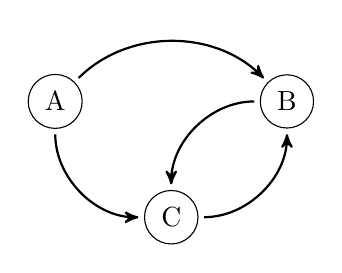
\begin{tikzpicture}[
roundnode/.style={circle, draw=black, thin},
]
%Nodes
\node[roundnode](C){C};
\node[above=of C](dummy){};

\node[roundnode](A)[left=of dummy]{A};

\node[roundnode](B)[right=of dummy]{B};

\path[pil] (A) edge [bend right=45] (C);
\path[pil] (B) edge [bend right=45] (C);
\path[pil] (C) edge [bend right=45] (B);
\path[pil] (A) edge [bend left=45] (B);

\end{tikzpicture}
\end{center}

\noindent Transition matrix
\begin{center}
\begin{tabular}{ |l|l|l|l| }
    \hline
      & A  & B  & C \\
    \hline
    A & 0  & 1  & 1  \\
    B & 0  & 0  & 1  \\
    C & 0  & 1  & 0  \\
    \hline
\end{tabular}
\end{center}

\noindent Transition probability matrix
\begin{center}
\begin{tabular}{ |l|l|l|l| }
    \hline
      & A    & B  & C \\
    \hline
    A & 0    & 0.5 & 0.5  \\
    B & 0    & 0   & 1    \\
    C & 0    & 1   & 0    \\
    \hline
\end{tabular}
\end{center}

\noindent Transition probability matrix with teleporting
\begin{center}
\begin{tabular}{ |l|l|l|l| }
    \hline
      & A    & B    & C      \\
    \hline
    A & 0.03  & 0.483 & 0.483  \\
    B & 0.03  & 0.03  & 0.933 \\
    C & 0.03  & 0.933 & 0.03  \\
    \hline
\end{tabular}
\end{center}

$$x = [1,0,0]$$
$$xP = [0.03, 0.48, 0.48]$$
$$xP^2 = [0.03, 0.48, 0.48]$$

\noindent \textbf{Question 4d}

\noindent Not in syllabus\\

\noindent \textbf{Question 4e}

\noindent Solution not provided

\end{multicols*}
\end{document}
